\documentclass[12pt]{extarticle}
\title{}
\author{Avinash Iyer}
\date{}
\usepackage[shortlabels]{enumitem}

%font setup
%
%\usepackage{newpxtext,eulerpx}

%paper setup
\usepackage{geometry}
\geometry{letterpaper, portrait, margin=1in}
\usepackage{fancyhdr}

%symbols
\usepackage{amsmath}
\usepackage{amsfonts}
\usepackage{mathtools}
\usepackage{hyperref}
\usepackage{gensymb}

\usepackage[T1]{fontenc}
\usepackage[utf8]{inputenc}

%chemistry stuff
\usepackage[version=4]{mhchem}
\usepackage{chemfig}

%plotting
\usepackage{pgfplots}
\usepackage{tikz}
\tikzset{middleweight/.style={pos = 0.5, fill=white}}
\tikzset{weight/.style={pos = 0.5, fill = white}}
\tikzset{lateweight/.style={pos = 0.75, fill = white}}
\tikzset{earlyweight/.style={pos = 0.25, fill=white}}

%\usepackage{natbib}

%graphics stuff
\usepackage{graphicx}
\graphicspath{ {./images/} }

%code stuff
%when using minted, make sure to add the -shell-escape flag
%you can use lstlisting if you don't want to use minted
%\usepackage{minted}
%\usemintedstyle{pastie}
%\newminted[javacode]{java}{frame=lines,framesep=2mm,linenos=true,fontsize=\footnotesize,tabsize=3,autogobble,}
%\newminted[cppcode]{cpp}{frame=lines,framesep=2mm,linenos=true,fontsize=\footnotesize,tabsize=3,autogobble,}

\usepackage{listings}
\usepackage{color}
\definecolor{dkgreen}{rgb}{0,0.6,0}
\definecolor{gray}{rgb}{0.5,0.5,0.5}
\definecolor{mauve}{rgb}{0.58,0,0.82}

\lstset{frame=tb,
	language=Java,
	aboveskip=3mm,
	belowskip=3mm,
	showstringspaces=false,
	columns=flexible,
	basicstyle={\small\ttfamily},
	numbers=none,
	numberstyle=\tiny\color{gray},
	keywordstyle=\color{blue},
	commentstyle=\color{dkgreen},
	stringstyle=\color{mauve},
	breaklines=true,
	breakatwhitespace=true,
	tabsize=3
}
% text + color boxes
\usepackage{tcolorbox}
\tcbuselibrary{breakable}
\newtcolorbox{problem}[1]{colback = white, title = {#1}, breakable}
\newtcolorbox{solution}{colback = white, colframe = black!75!white, title = Solution, breakable}
%including PDFs
\usepackage{pdfpages}
\setlength{\parindent}{0pt}

\pagestyle{fancy}
\fancyhf{}
\rhead{Avinash Iyer}
\lhead{Applications of Graph Theory: Homework 1}
\begin{document}{
  \begin{problem}{Exercise 3}
    Suppose that four houses are under construction and each house must be provided with a connection of each of two utilities. Under the same conditions as the Three Houses and Three Utilities problem, can these conditions be satisfied for this Four Houses and Two Utilities Problem?
    \tcblower
    \begin{center}
      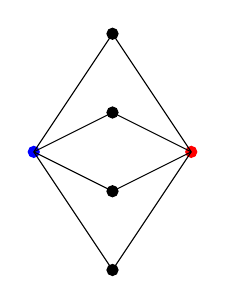
\begin{tikzpicture}
        \filldraw[blue] (-1,0) circle (2pt);
        \filldraw[red] (1,0) circle (2pt);
        \filldraw (0,1.5) circle (2pt)
        (0,0.5) circle (2pt)
        (0,-0.5) circle (2pt)
        (0,-1.5) circle (2pt);
        \draw (-1,0) -- (0,1.5);
        \draw (-1,0) -- (0,0.5);
        \draw (-1,0) -- (0,-1.5);
        \draw (-1,0) -- (0,-0.5);
        \draw (1,0) -- (0,1.5);
        \draw (1,0) -- (0,0.5);
        \draw (1,0) -- (0,-1.5);
        \draw (1,0) -- (0,-0.5);
      \end{tikzpicture}
    \end{center}
  \end{problem}
  \begin{problem}{Exercise 5}
    For the two polyhedra shown below, determine the number $V$ of vertices, the number $E$ of edges, and the number $F$ of faces. Show that the Euler Polyhedron Formula holds in each case.
    \begin{center}
      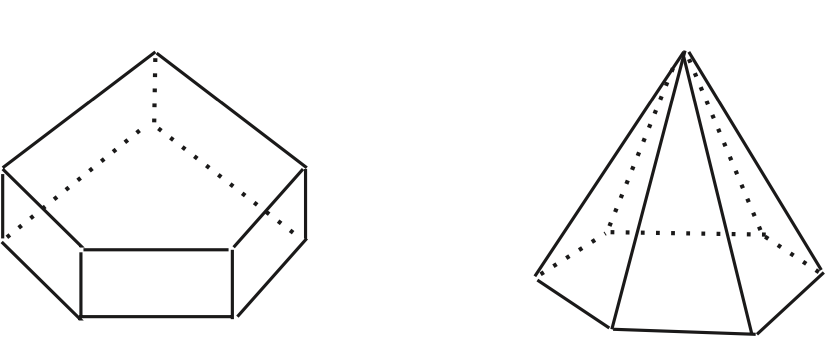
\includegraphics[width=5cm]{exercise_5}
    \end{center}
    \tcblower
    For the first polyhedron, we have $V = 10$, $E = 15$, $F = 7$, so $V-E+F = 2$.\\

    For the second polyhedron, we have $V = 7$, $E = 12$, and $F = 7$, so $V-E+F = 2$.
  \end{problem}
  \begin{problem}{Exercise 8a}
    Show that a knight's tour is not possible on a $4\times 4$ chessboard.
    \tcblower
    \begin{center}
      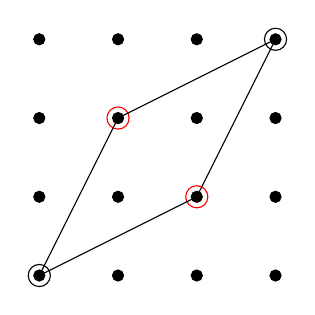
\begin{tikzpicture}
        \filldraw (0,0) circle (2pt)
              (0,1) circle (2pt)
              (0,2) circle (2pt)
              (0,3) circle (2pt)
              (1,0) circle (2pt)
              (1,1) circle (2pt)
              (1,2) circle (2pt)
              (1,3) circle (2pt)
              (2,0) circle (2pt)
              (2,1) circle (2pt)
              (2,2) circle (2pt)
              (2,3) circle (2pt)
              (3,0) circle (2pt)
              (3,1) circle (2pt)
              (3,2) circle (2pt)
              (3,3) circle (2pt);
        \draw (0,0) circle (4pt);
        \draw (3,3) circle (4pt);
        \draw[red] (2,1) circle (4pt)
                    (1,2) circle (4pt);
        \draw (0,0) -- (2,1) -- (3,3) -- (1,2) -- cycle;
      \end{tikzpicture}
    \end{center}
    In order to perform a knight's tour, one must visit the two squares circled in black, implying that the knight must pass through the two squares circled in red. However, since these form a cycle, this means that for the knight to visit any other square, it must visit the squares in red more than once.
  \end{problem}
  \begin{problem}{Exercise 10}
    Eight coins are placed on the nine squares of a $3\times 3$ chessboard, at most one coin per square. Therefore, exactly one square does not contain a coin. The nine possible configurations are shown below, where the configuration labeled $(i,j)$ indicates that the square without a coin is located in row $i$ and column $j$. If a coin in configuration $(i,j)$ can be moved horizontally or vertically one square to the vacant square in that configuration to produce the configuration $(k,\ell)$, we say that the configuration $(i,j)$ can be transformed into configuration $(k,\ell)$. Observe that if configuration $(i,j)$ can be transformed into configuration $(k,\ell)$, then it can be transformed into configuration $(i,j)$. Show that this situation can be represented by a graph.
    \begin{center}
      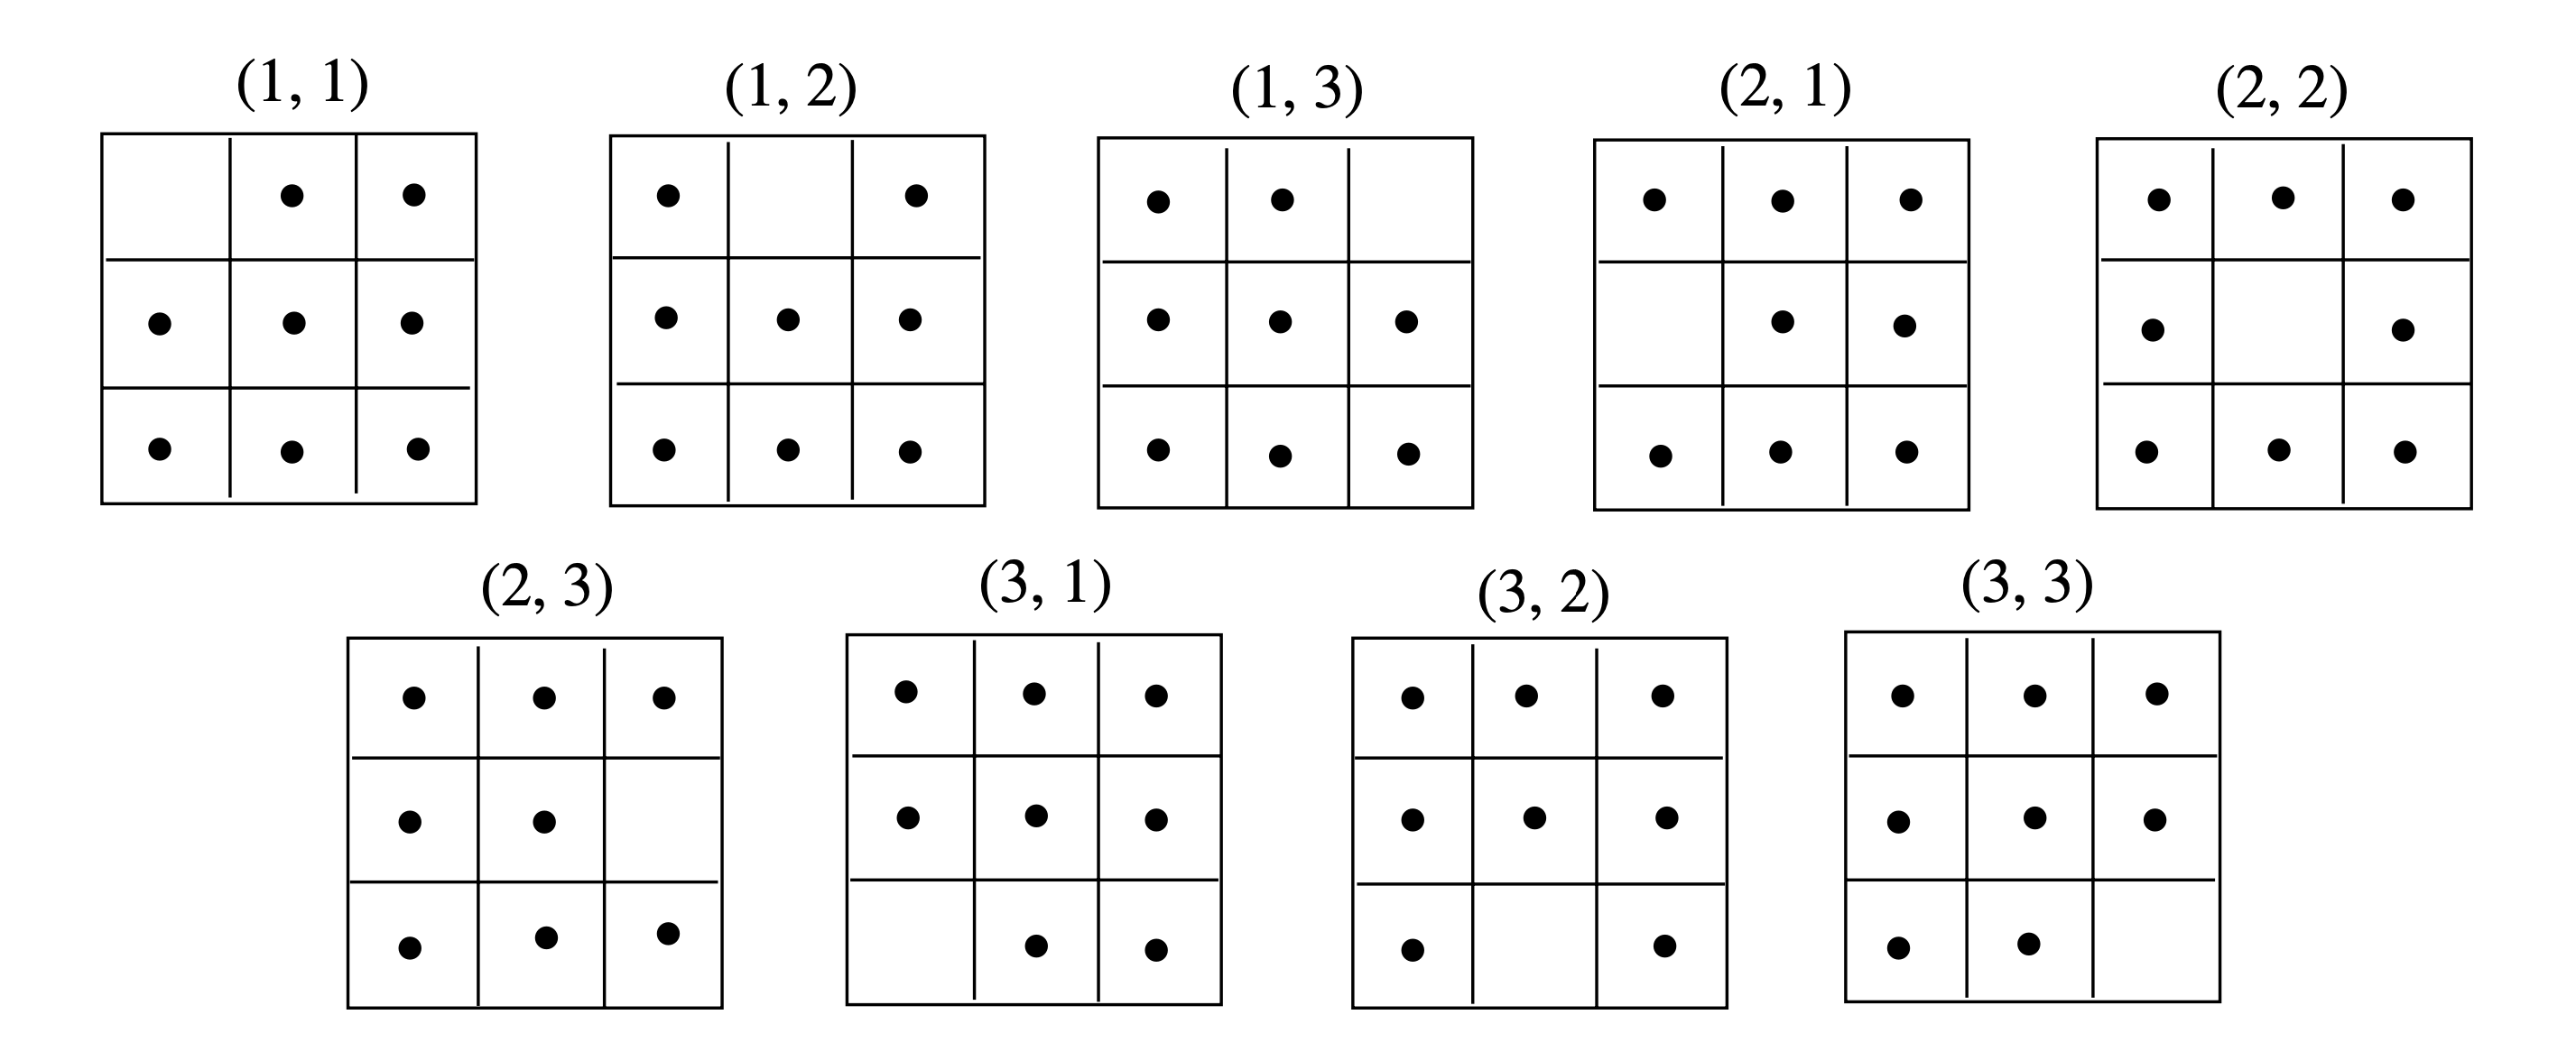
\includegraphics[width=10cm]{exercise_10}
    \end{center}
    \tcblower
    \begin{center}
      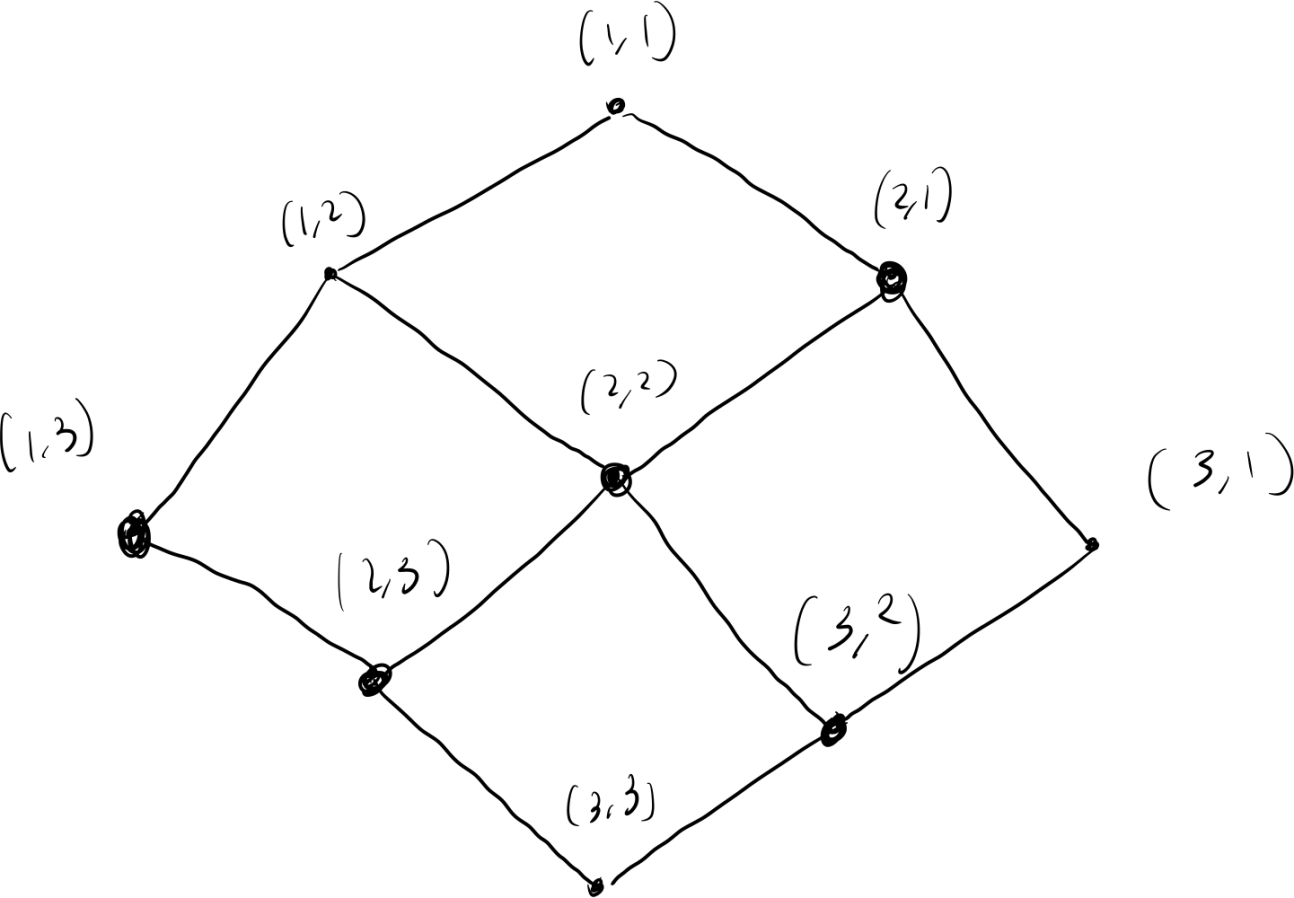
\includegraphics[width=7cm]{exercise_10_solution}
    \end{center}
  \end{problem}
  \begin{problem}{Exercise 11}
    Suppose instead that only one coin is placed on one of these squares. The configuration $(i,j)$, where $i,j\in \{1,2,3\}$, indicates that the coin is on the square in row $i$ and column $j$. The coin in configuration $(i,j)$ can be moved one square horizontally or one square vertically to be transformed into the configuration $(k,\ell)$. Draw the graph that represents this situation.
    \tcblower
    The graph is the same as that of the previous problem, as instead of the ``hole'' in the board, we are using the coin in place of the hole. Therefore, the graph looks like the following.
    \begin{center}
      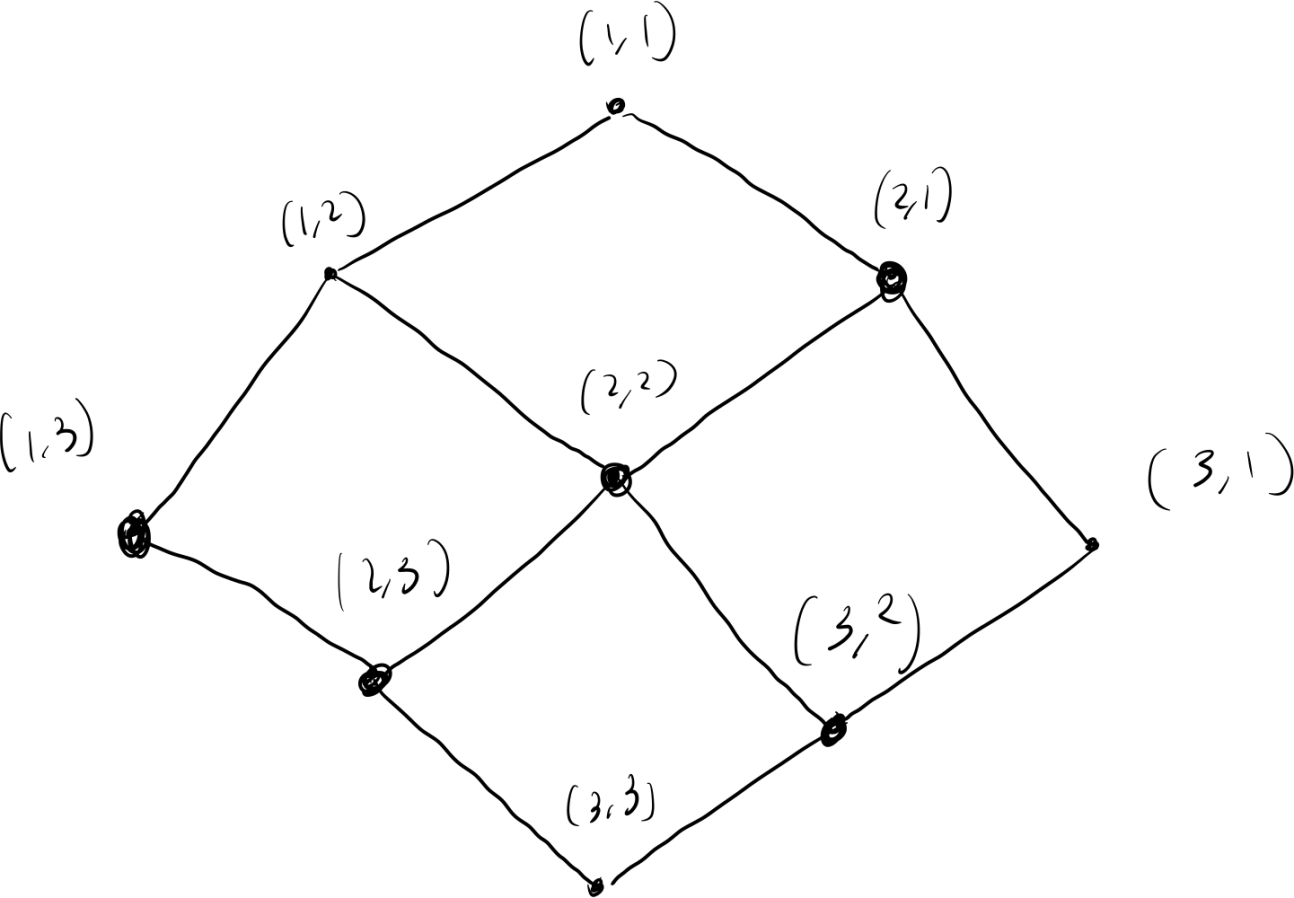
\includegraphics[width=7cm]{exercise_10_solution}
    \end{center}
  \end{problem}
  \begin{problem}{Exercise 14}
    During the holidays, a community has three decorated trees located in a row on a platform where the lights on each tree are either all blue or all silver. Every minute the lights on one of these trees change color (from all blue to all silver or from all silver to all blue). Draw a graph that represents this situation.
    \tcblower
    Let $1$ represent a tree with silver lights and let $0$ represent a tree with blue lights. Then, we can represent the tree as the following:
    \begin{center}
      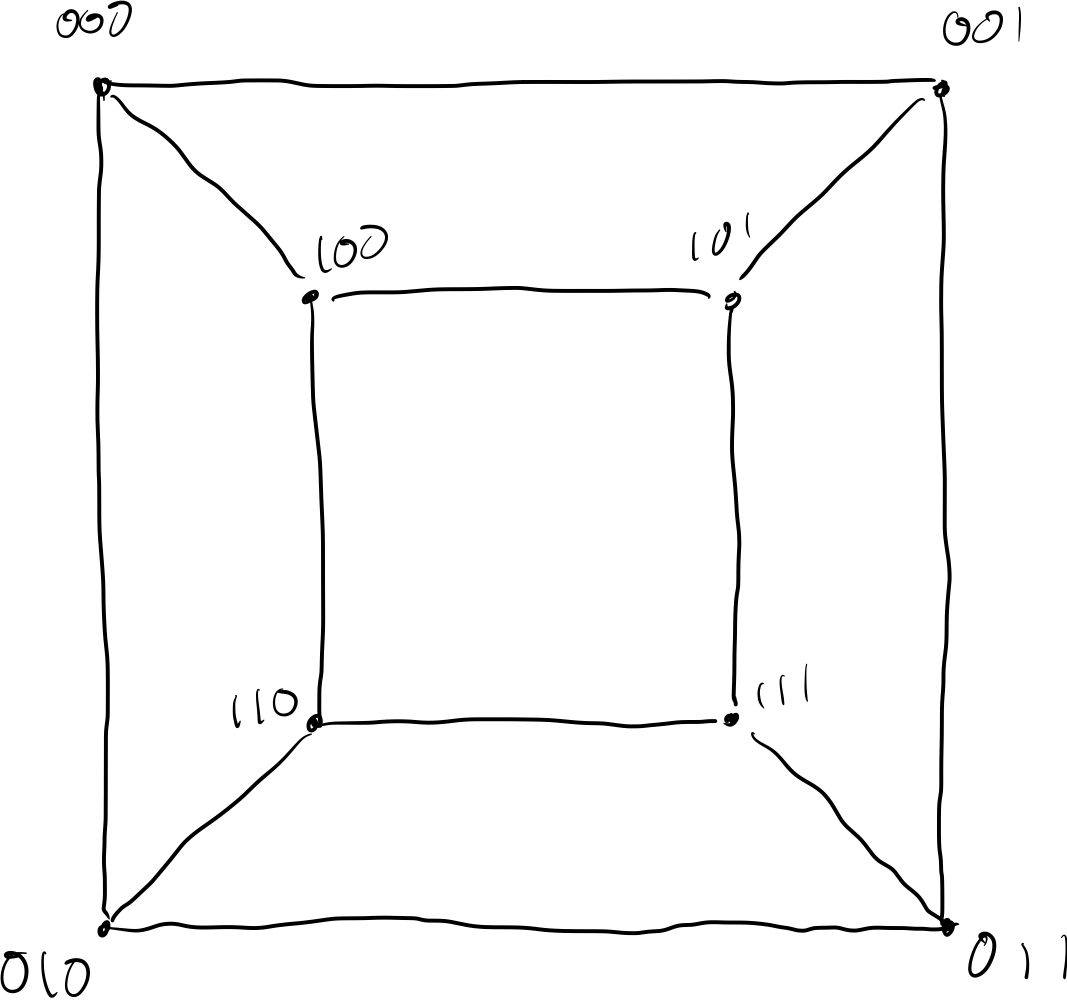
\includegraphics[width=7cm]{exercise_14_solution}
    \end{center}
  \end{problem}
  \begin{problem}{Exercise 19}
    The figure below shows the traffic lanes at the intersection of two busy streets. When a vehicle approaches this intersection, it could be in one of the nine lanes $L_1,\dots,L_9$. This intersection has a traffic light that informs drivers in vehicles in the various lanes when they are permitted to proceed through the intersection. To be sure, there are pairs of lanes containing vehicles that should not enter the intersection at the same time, such as $L_1$ and $L_7$. However, there would be no difficulty for vehicles in $L_1$ and $L_5$, for example, to drive through this intersection at the same time. Represent this situation by a graph.
    \begin{center}
      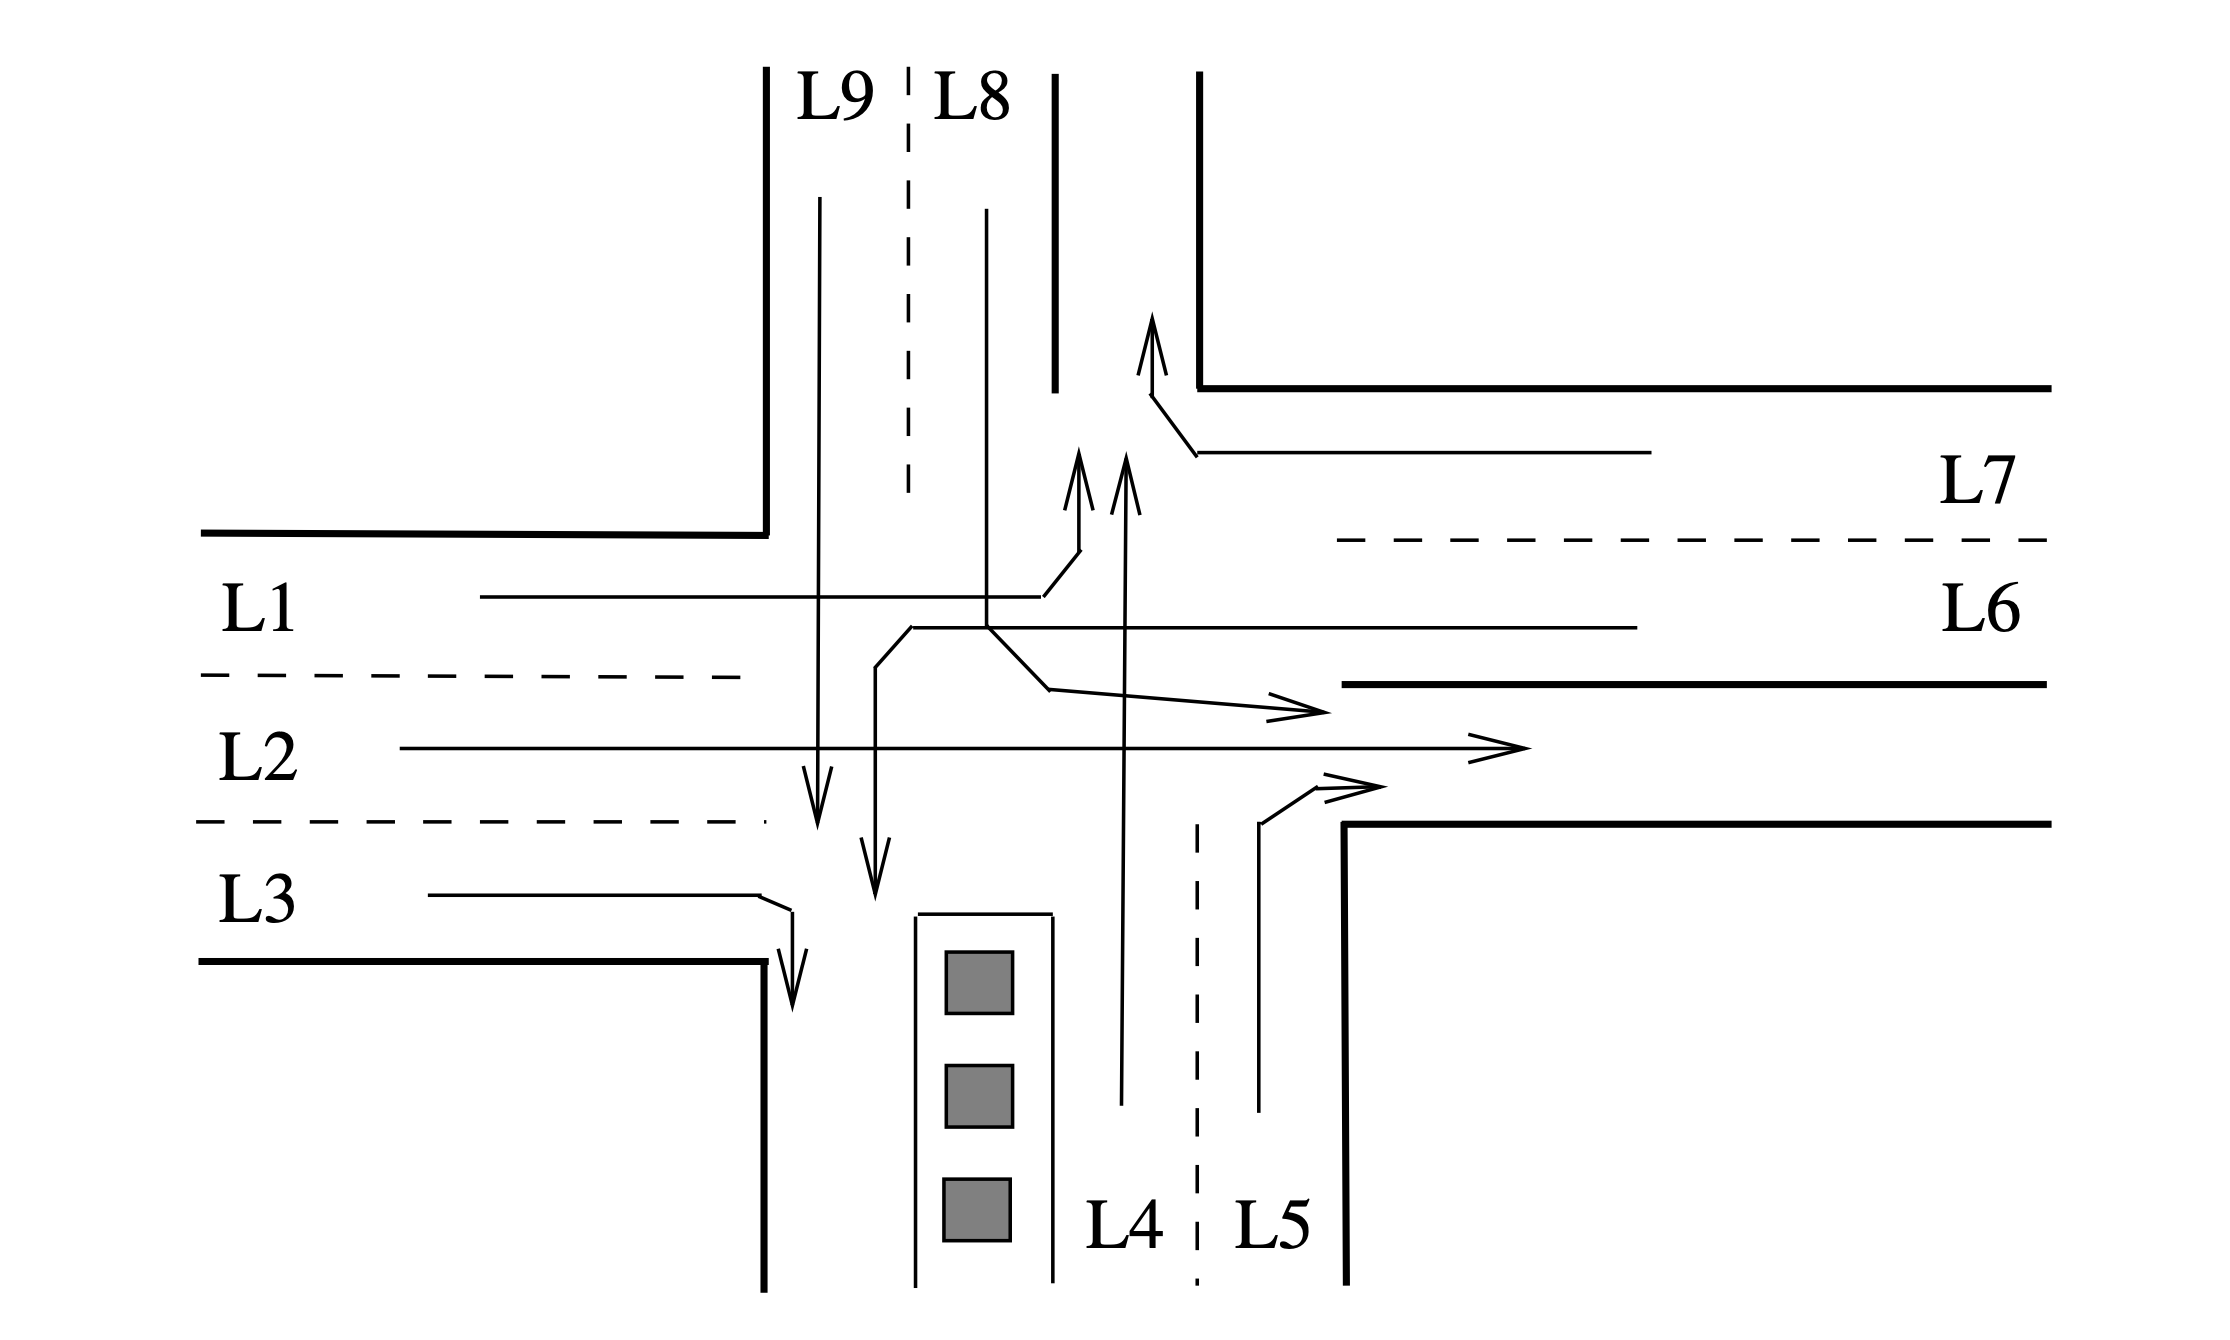
\includegraphics[width=10cm]{exercise_19}
    \end{center}
    \tcblower
    \begin{center}
      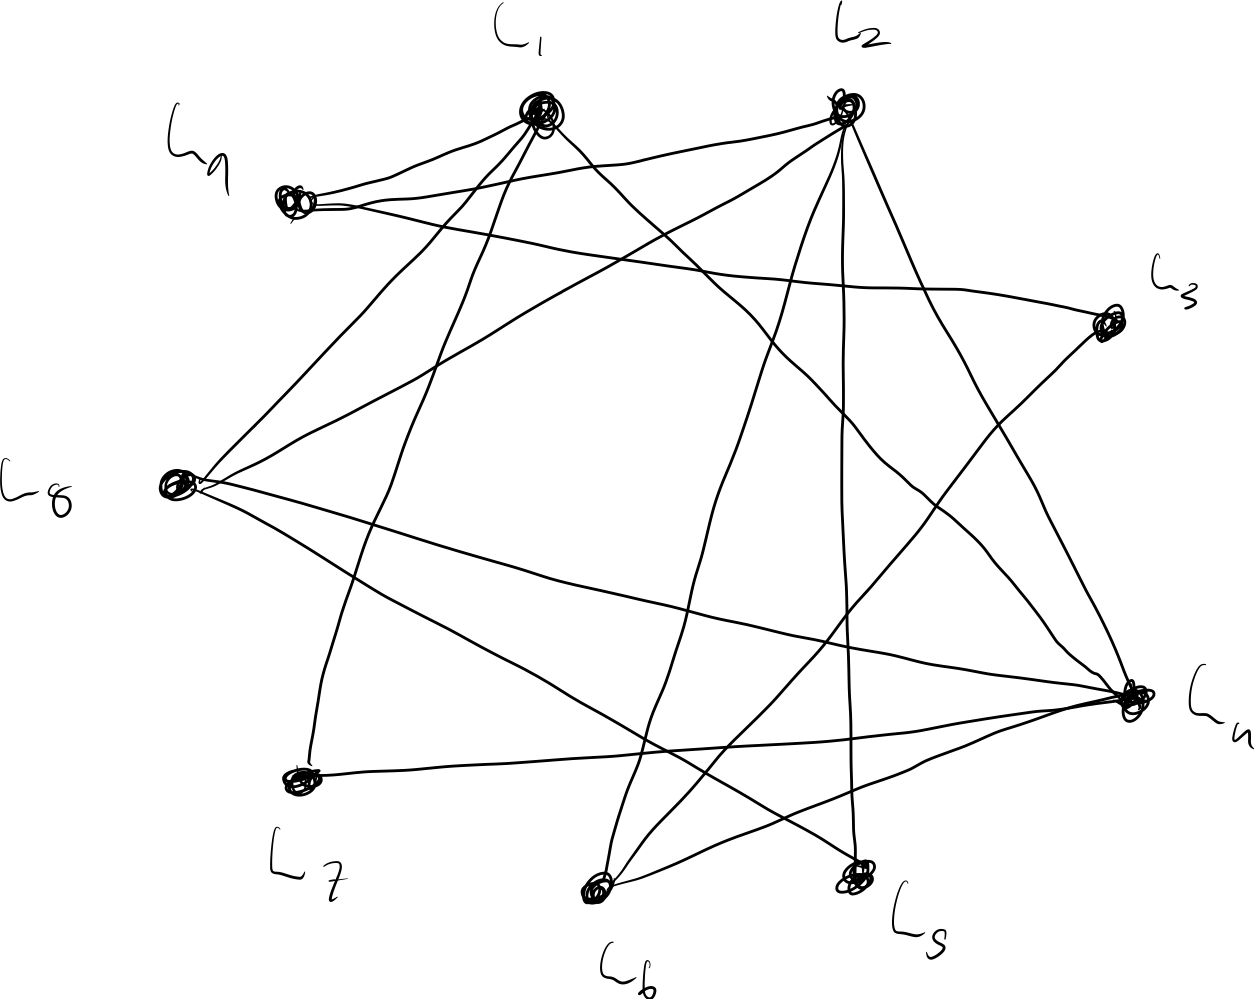
\includegraphics[width=7cm]{exercise_19_solution}
    \end{center}
  \end{problem}
}\end{document}
